\section{Модели и спецификация требований к программному средству}
\label{sec:funcreq}

\subsection{Функциональная модель программного средства}
\label{sec:funcreq:funcmodel}

С оглядкой на существующие реализации рассматриваемой задачи определим варианты использования програмного средства.

\begin{figure}[ht]
\centering
    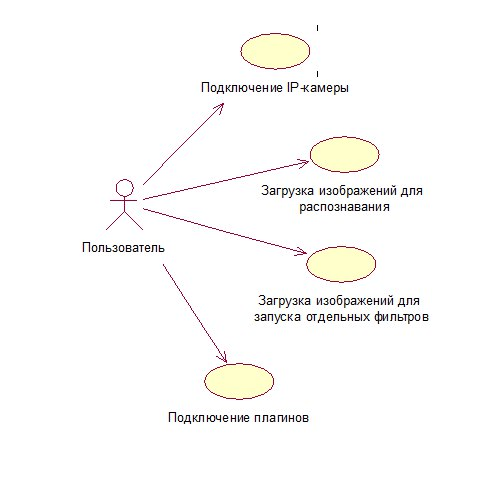
\includegraphics[scale=1]{func_model.jpg}  
    \caption{Диаграмма вариантов использования}
  \label{fig:funcreq:funcmodel}
\end{figure}

На основе вариантов использования для разрабатываемого программного средства формируется следующий набор функциональных требований:
\begin{itemize}
	\item Подключение и обработка видеопотока с IP камеры
	\item Загрузка изображения для распознавания.
	\item Загрузка изображения для запуска отдельных, выбранных пользователе фильтров.
	\item Подключение плагинов для интеграции с существующей инфраструктурой.
\end{itemize}

\subsection{Спецификация требований к программному средству}
\label{sec:fucreq:specification}

\subsubsection{}
Подключение IP камер. Требования:
\begin{itemize}
	\item Возможность добавить камеру должна быть как с командной строки так и из пользовательского интерфейса
	\item Адреса добавленных IP камер должны сохранятся и при перезапуске сервера, сервер должен снова подключится к камерам
	\item Должна быть возможность добавить несколько IP камер.
	\item У каждой IP камеры кроме имени должен быть псевдоним, который будет передаваться вместе с результатами распознавания в плагины. 
\end{itemize}

\subsubsection{}
Загрузка картинки для распознавания. Требования:
\begin{itemize}
	\item Возможность загрузить изображение на сервер для распознавания.
	\item Поддержка форматов PNG и JPEG.
\end{itemize}


